\chapter{Gestione della memoria}
\textit{Cosa si intende per gestione della memoria (RAM) e perché gestirla?} La memoria oggi è a basso costo, e con trend in diminuzione, tuttavia, ciò è più che bilanciato dal fatto che le moderne applicazioni richiedono sempre maggiore memoria. Se si lasciasse a ciascun processo la gestione della propria memoria, ogni processo userebbe semplicemente tutta la memoria a disposizione. Si potrebbe allora imporre dei limiti di memoria a ciascun processo ma diventa difficile per un programmatore scrivere un programma che rispetti tali limiti. Quindi i compiti di gestione della memoria passano al sistema operativo che illude i processi di avere tutta la memoria a disposizione eseguendo degli swap (scambi) di blocchi di dati nella memoria secondaria. Questa gestione di I/O è ovviamente più lenta del processore, pertanto il sistema operativo deve pianificare lo swap in modo intelligente, così da massimizzare l'efficienza del processore e gestire la memoria affinché ci sia sempre un numero ragionevole di processi pronti all'esecuzione.

\section{Requisiti per la gestione della memoria}
I requisiti essenziali per la gestione nella memoria sono: rilocazione, protezione, condivisione, organizzazione logica e organizzazione fisica. Vediamoli in dettaglio:
\begin{itemize}
    \item Il concetto di \textit{rilocazione} prevede che il programmatore non deve sapere in quale zona della memoria il programma viene caricato. Infatti potrebbe essere swappato su disco, e al ritorno in memoria principale potrebbe essere in un'altra posizione, potrebbe avere alcune pagine in RAM e altre su disco... I riferimenti alla memoria, inoltre, devono essere tradotti nell'indirizzo fisico “vero” attraverso una fase di preprocessing o a run-time.
    
    Possiamo intendere un programma come formato da una zona per il programma scritto in linguaggio macchina, una per i dati (variabili globali) e una per lo stack delle chiamate (variabili locali), vedi Figura \ref{fig:indirizzi-programmi}. Gli indirizzi del programma possono essere o istruzioni di salto (Branch instruction, ad esempio \verb|jump|) o riferiti ai dati (Reference to data, ad esempio \verb|lw, sw|...). Tutti questi indirizzi devono essere ricalcolati se il sistema operativo vuole garantire la rilocazione.

    Ogni programma, in compilazione, viene diviso in una serie di moduli compilati separatamente che vengono uniti da un \textit{liker} per creare un programma eseguibile chiamato \textit{Load module}. Il load module può essere direttamente caricato in RAM tramite un \textit{Loader}, vedi Figura \ref{fig:indirizzi-programmi}. A questo punto gli indirizzi di memoria vengono determinati o nel momento in cui il programma viene caricato in memoria (\textit{preprocessing}) o a \textit{run-time}, ovvero nel momento in cui si fa un riferimento alla memoria. Gli indirizzi possono essere di tre tipi: \textit{indirizzi logici} dove il riferimento in memoria è indipendente dall'attuale posizionamento del programma in memoria, \textit{indirizzi relativi} dove il riferimento è espresso come uno spiazzamento rispetto ad un qualche punto noto e \textit{indirizzi fisici o assoluti} dove il riferimento è quello effettivo alla locazione di memoria.

    \begin{figure}
        \centering
        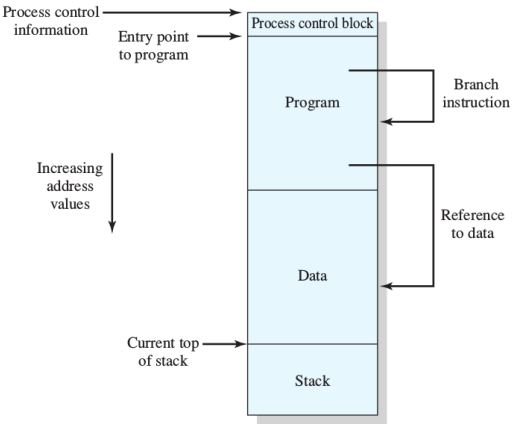
\includegraphics[width=0.42\linewidth]{images/indirizzi-programmi.JPG}
        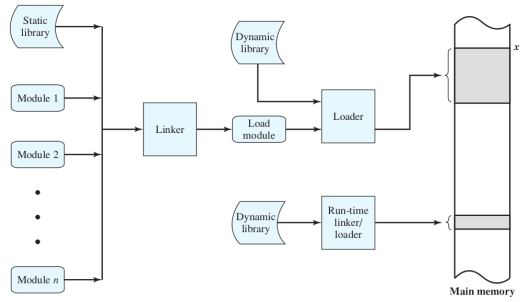
\includegraphics[width=0.57\linewidth]{images/indirizzi-programmi2.JPG}
        \caption{Indirizzi nei programmi}
        \label{fig:indirizzi-programmi}
    \end{figure}

    \begin{Example}{Rilocazione di indirizzi relativi}{}
        Ipotizziamo di eseguire l'istruzione \verb|jump| all'indirizzo 400, essendo un indirizzo relativo, l'hardware del compilatore "sa" che quel valore deve essere sommato al Base register per ottenere il riferimento effettivo.
        
        \begin{minipage}{\textwidth}
            \centering
            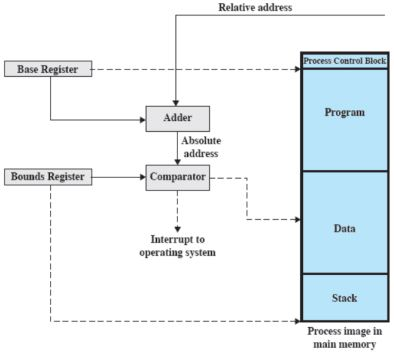
\includegraphics[width=0.5\textwidth]{images/rilocazione-indirizzi-relativi.JPG}
            \label{fig:rilocazione-indirizzi-relativi}
        \end{minipage}
        
        Il \textit{Base register} (registro base) indica l'indirizzo di partenza del processo, mentre il \textit{Bounds register} (registro limite) rappresenta l'indirizzo di fine del processo. I valori per questi registri vengono settati nel momento in cui il processo viene posizionato in memoria e vengono mantenuti nel PCB del processo. Il valore del registro base viene aggiunto al valore dell'indirizzo relativo per ottenere l'indirizzo assoluto, il risultato viene confrontato con il registro limite e se va oltre, viene generato un interrupt per il sistema operativo.
    \end{Example}

    \item Per \textit{protezione} si intende che i processi non devono poter accedere a locazioni di memoria di un altro processo, a meno che non siano autorizzati. A causa della rilocazione, deve essere necessariamente fatto a tempo di esecuzione con aiuto hardware.

    \item Il contrario della protezione è la \textit{condivisione}, che deve permettere a più processi di accedere alla stessa zona di memoria, ovviamente solo se è effettivamente utile allo scopo perseguito dai processi. Un caso tipico è quando si creano più processi eseguendo lo stesso codice sorgente e, finché questi processi restano in esecuzione, è più efficiente che condividano il codice sorgente, visto che è lo stesso.

    \item A livello hardware, le memorie sono organizzata in modo lineare, ma a livello software, i programmi sono scritti in moduli, che possono essere compilati separatamente, avere diversi permessi... Secondo l'\textit{organizzazione logica} il sistema operativo deve essere un tramite tra la visione ad alto livello dei programmatori e quella hardware delle memorie.

    \item L'\textit{organizzazione fisica} è un altro compito del sistema operativo che deve gestire il flusso tra RAM e memoria secondaria.
    
\end{itemize}

\section{Partizionamento della memoria}
In questa sezione verranno presentate diversi tipi di strategie che sono state utilizzate nel corso degli anni per la gestione della memoria, fino ad arrivare alla memoria virtuale che è quella utilizzata ancora oggi.

Uno dei primi metodi per la gestione della memoria è il \textit{partizionamento} che può essere di vari tipi: fisso, dinamico,  semplice, segmentazione semplice, paginazione con memoria virtuale, segmentazione con memoria virtuale. È utile comprendere queste tecniche di partizionamento perché rappresentano le fondamenta della gestione della memoria, da cui la memoria virtuale stessa trae origine.

\subsection*{Partizionamento fisso}

\begin{wrapfigure}{r}{0.25\linewidth}
    \vspace{-10pt}
    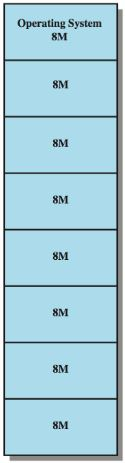
\includegraphics[width=0.48\linewidth]{images/partizionamento-fisso-uniforme.JPG}
    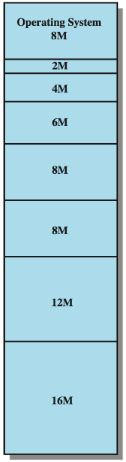
\includegraphics[width=0.483\linewidth]{images/partizionamento-fisso-variabile.JPG}
    %\caption{Partizionamento fisso uniforme e variabile}
    \label{fig:partizionamento-fisso}
    \vspace{-20pt}
\end{wrapfigure}

Nel \textit{partizionamento fisso uniforme}, dopo l'accensione del sistema, la memoria RAM viene divisa in partizioni di uguale lunghezza. Se un processo ha una dimensione minore o uguale della misura di una partizione, allora può essere caricato in una partizione libera. Il sistema operativo può togliere un processo da una partizione e spostarlo su disco.

Da questo tipo di partizionamento nascono notevoli problematiche date dal fatto che un programma potrebbe non entrare in una partizione oppure c'è un uso inefficiente della memoria perché ogni programma, anche il più piccolo, occupa un'intera partizione, causando frammentazione interna\footnote{Quando un programma riceve un certo quantitativo di memoria, ma non utilizza completamente tutto lo spazio assegnato, la porzione di memoria inutilizzata all'interno di quel blocco è chiamata frammentazione interna.}.

Con il \textit{partizionamento fisso variabile} vengono mitigati alcuni problemi del partizionamento fisso uniforme. Infatti la memoria viene sempre divisa in più parti fisse ma ogni partizione ha una dimensione diversa (maggiore o minore) rispetto alle altre.

E' necessario, in questo tipo di partizionamento, un algoritmo di posizionamento per decidere in quale blocco collocare il nuovo processo. La soluzione più ovvia è inserire un processo nella partizione più piccola che può contenerlo in modo da minimizzare la quantità di spazio sprecato.

Restano comunque dei problemi irrisolti dato che c'è un numero massimo di processi in memoria principale, corrispondente al numero di partizioni deciso inizialmente, e se ci sono molti processi piccoli, la memoria verrà usata in modo inefficiente.

\subsection*{Partizionamento dinamico}
Visti i problemi incontrati nel partizionamento fisso, si è deciso di passare al \textit{partizionamento dinamico}, dove le partizioni variano sia in misura che in quantità e per ciascun processo viene allocata esattamente la quantità di memoria che serve.

\begin{Example}{Partizionamento dinamico}{}
    In un sistema operativo con 64M di RAM con partizionamento dinamico abbiamo 8M di memoria per il kernel e i restanti 56M sono vuoti. In un certo istante di tempo arrivano in sequenza tre processi: $P_1$ da 20M, $P_2$ da 14M e $P_3$ da 18M che vengono allocati in tre partizioni diverse. Supponiamo che arrivi un processo $P_4$ da 8M, non essendoci abbastanza spazio per una nuova partizione, il sistema operativo decide che $P_4$ è più importante di $P_2$ che lascia parte del suo spazio al nuovo processo. Ovviamente $P_2$ non viene terminato ma viene copiato su disco finché il sistema operativo non decide di riportarlo in RAM.
    \begin{minipage}{\textwidth}
        \centering
        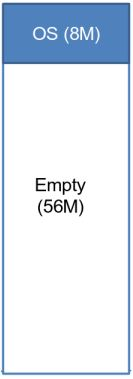
\includegraphics[width=0.130\textwidth]{images/esempio-partizionamento-dinamico1.JPG}
        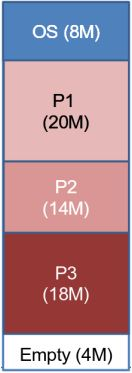
\includegraphics[width=0.130\textwidth]{images/esempio-partizionamento-dinamico2.JPG}
        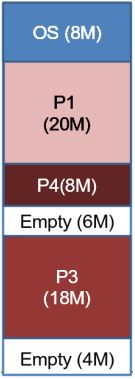
\includegraphics[width=0.131\textwidth]{images/esempio-partizionamento-dinamico3.JPG}
        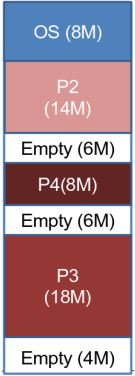
\includegraphics[width=0.132\textwidth]{images/esempio-partizionamento-dinamico4.JPG}
        \label{fig:esempio-partizionamento-dinamico}
    \end{minipage}

    Da notare che nel caso in cui arriva un nuovo processo da 8M, c'è abbastanza memoria ma non essendo contigua bisogna swappare su disco un processo.
\end{Example}

Anche con questo tipo di partizione ci problemi dovuti alla frammentazione esterna\footnote{Si verifica quando ci sono zone di memoria libera tra le regioni occupate dai processi, ma tali regioni libere non sono sufficientemente grandi o contigue per soddisfare le richieste di memoria di un nuovo processo.} che si può risolvere compattando i processi di modo che siano contigui. Inoltre, il sistema operativo deve decidere a quale blocco libero assegnare un processo. L'algoritmo più ovvio è il \textit{best-fit} che sceglie il blocco la cui misura è la più vicina a quella del processo da posizionare, nonostante l'apparenza, è quello con risultati peggiori perché lascia dei frammenti molto piccoli e costringe a fare spesso la compattazione. Un'alternativa è il \textit{first-fit} che scorre la memoria dall'inizio e il primo blocco con abbastanza memoria viene subito scelto, è molto veloce anche se tende a riempire solo la prima parte della memoria e in media è la soluzione migliore. Un'ultima possibilità sarebbe il \textit{next-fit} che opera come il first-fit, ma anziché partire ogni volta dall'inizio, parte dall'ultima posizione assegnata ad un processo e tende ad assegnare più spesso il blocco alla fine della memoria, che è quello più grosso.

\subsection*{Buddy System}
Il \textit{Buddy System} (sistema del compagno) è un compromesso tra partizionamento fisso e dinamico. Sia $2^U$ la dimensione dello user space ed $s$ la dimensione di un processo da mettere in RAM, si dimezza lo spazio fino a trovare un $X$ tale che $2^{X-1}<s\leq 2^X$, con $L\leq X\leq U$, $L$ serve per dare un lower bound in modo da non creare partizioni troppo piccole. In questo modo si trovano due diverse partizioni di cui una è utilizzata per il processo. Ovviamente, in questo sistema, occorre tener presente le porzioni già occupate e quando un processo finisce, se il buddy è libero si può fare una fusione.

\begin{Example}{Buddy System}{}
In un sistema con 1M arriva un processo A che richiede 100K, vengono create le partizioni 512K, 256K e 128K e viene inserito il processo nella partizione da 128K. Supponiamo che arrivino tre processi B, C e D da 240K, 64K e 256K il primo e l'ultimo vengono inseriti rispettivamente nei blocchi da 128K e 256K e, per il secondo, viene effettuata la divisione del blocco di 128K in due da 64K e inserito il processo al suo interno. 
    
Ora nel caso in cui vengono terminati i processi A e B, si dovrebbero fondere i blocchi liberati con i loro compagni (buddy) per creare delle porzioni più grandi, ma in entrambe i casi non è fattibile perché non vengono creati blocchi liberi da 256K per A e 512K per B. Quindi vengono semplicemente liberate delle partizioni di memoria per il nuovo processo E da 75K. Diversamente accade quando vengono terminati i processi C ed E, perché vengono fusi i quattro blocchi liberi di memoria in uno da 512K.
    \begin{minipage}{\textwidth}
        \centering
        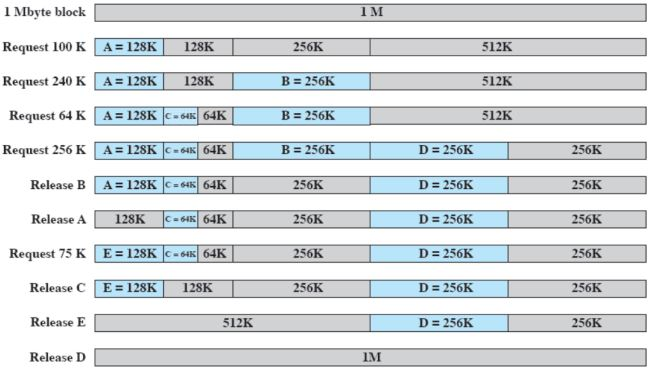
\includegraphics[width=0.7\textwidth]{images/esempio-buddy-system.JPG}
        \label{fig:esempio-buddy-system}
    \end{minipage}
\end{Example}

\section{Paginazione e segmentazione}
Per arrivare alla paginazione e segmentazione moderne, ovvero con memoria virtuale, dobbiamo prima analizzare quelle semplici. 
\subsection*{Paginazione semplice}
La paginazione semplice probabilmente non è mai stata usata, ma è importante per introdurre la memoria virtuale. In questo sistema sia la memoria che i processi vengono partizionati in piccoli pezzi di grandezza uguale, i pezzi di processi sono chiamati \textit{pagine} e i pezzi di memoria sono chiamati \textit{frame}. Ogni pagina, per essere usata, dev'essere collocata in un frame e, in generale, una pagina può essere posizionata in un qualunque frame. E' necessario quindi che i sistemi operativi mantengono una \textit{tabella delle pagine} per ogni processo dove, per ogni pagina del processo, questa tabella indica in quale frame effettivo si trova, quando si genera un process switch, la tabella delle pagine del nuovo processo deve essere ricaricata. A questo punto, gli indirizzi di memoria relativi vengono modificati a favore di indirizzi contenenti un numero di pagina e uno spiazzamento al suo interno.

\begin{Example}{Paginazione semplice}{}
    La RAM è divisa in 15 frame e, in un certo istante di tempo, arrivano 3 processi A,B e C con rispettivamente 4,3 e 4 pagine che richiedono altrettanti frame per essere caricati. Supponiamo che termina il processo B e arriva un processo D con 5 pagine, se stessi usando il partizionamento dinamico il processo non sarebbe caricato senza compattazione, con la paginazione questo problema non sussiste perché le prime 3 pagine vengono collocate nei 3 frame disponibili e le altre 2 a seguire dopo il terzo processo.

    \begin{minipage}{\textwidth}
        \centering
        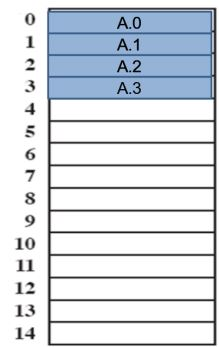
\includegraphics[width=0.143\textwidth]{images/esempio-paginazione-semplice.JPG}
        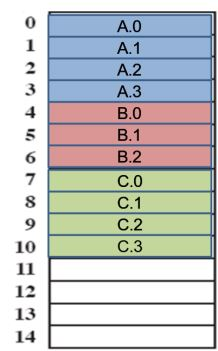
\includegraphics[width=0.143\textwidth]{images/esempio-paginazione-semplice2.JPG}
        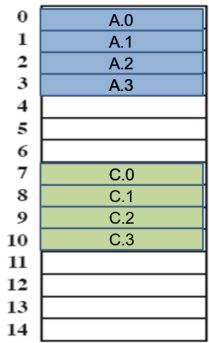
\includegraphics[width=0.14\textwidth]{images/esempio-paginazione-semplice3.JPG}
        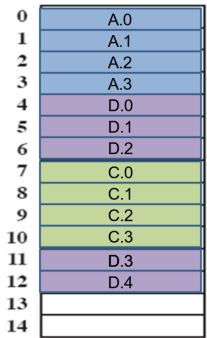
\includegraphics[width=0.14\textwidth]{images/esempio-paginazione-semplice4.JPG}
        \label{fig:esempio-paginazione-semplice}
    \end{minipage}
\end{Example}

\begin{Example}{Traduzione della tabella delle pagine}{}
    Supponiamo che la dimensione di una pagina sia 100 bytes e che la RAM dell'esempio precedente è di 1400 bytes in totale. Inoltre, i processi A, B, C e D richiedono rispettivamente 400, 300, 400 e 500 bytes. Nelle istruzioni dei processi, i riferimenti alla RAM sono relativi all'inizio del processo, quindi, ad esempio, per D ci saranno solo riferimenti compresi nell'intervallo [0, 499].

    Supponiamo ora che attualmente il processo D sia in esecuzione, e che occorra eseguire l'istruzione \verb|j 343|, bisogna prima capire in quale pagina di D si trova 343, basta fare $343/100=3$. Poi occorre guardare la tabella delle pagine di D, la 3$^a$ pagina corrisponde all'11° frame di RAM. Il frame 11 ha indirizzi che vanno da 1100 a 1199: basta fare $343 mod 100 = 43$, l'indirizzo vero è pertanto $11*100 + 43 = 1143$.
    \begin{osservation}
        Con l'hardware dei calcolatori, bisogna usare la base 2, quindi anche la dimensione delle pagine è una potenza di 2.
    \end{osservation}
\end{Example}

Con la paginazione, gli indirizzi ci forniscono due informazioni: una prima parte di bit indica il numero di pagina nella tabella delle pagine e una seconda parte indica l'offset. Basterà quindi affiancare il numero del frame con quello dell'offset per ottenere l'indirizzo fisico.

\begin{figure}[h]
    \centering
    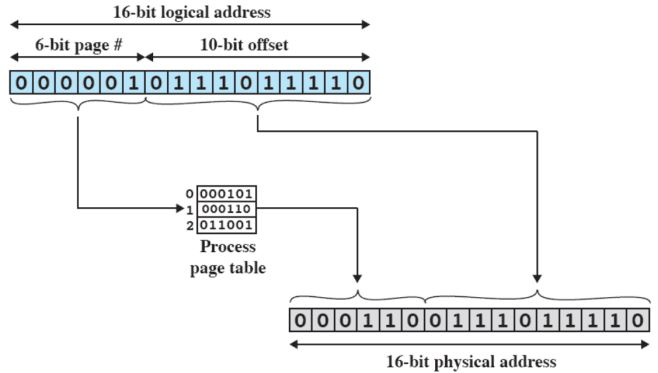
\includegraphics[width=0.7\linewidth]{images/esempio-paginazione.JPG}
    \caption{Esempio di indirizzi di paginazione}
    \label{fig:esempio-paginazione}
\end{figure}

\subsection*{Segmentazione semplice}
La segmentazione prevede che un programma può essere diviso in segmenti con lunghezza variabile e un limite massimo della dimensione. In questo senso è simile al partizionamento dinamico ma con una differenza fondamentale: il programmatore (o il compilatore) devono gestire esplicitamente la segmentazione dicendo quanti segmenti ci sono e qual è la loro dimensione per metterli effettivamente in RAM.

Per tradurre un indirizzo logico in uno fisico con la segmentazione, uso i primi bit dell'indirizzo per ottenere il numero di pagina dalla tabella dei segmenti, da questa estraggo il valore di inizio del processo per sommarlo all'offset (ultimi bit dell'indirizzo logico).

\begin{figure}[h]
    \centering
    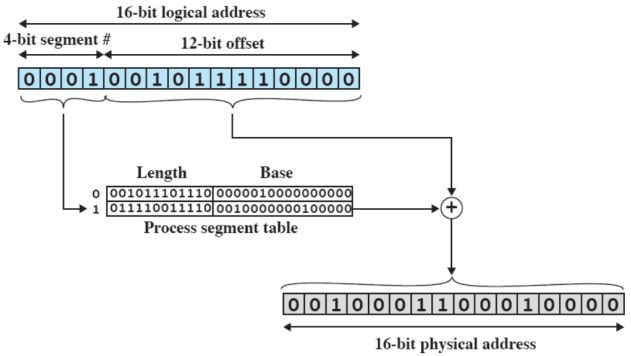
\includegraphics[width=0.7\linewidth]{images/segmentazione.JPG}
    \caption{Esempio di indirizzi di segmentazione}
    \label{fig:segmentazione}
\end{figure}

\section{Memoria virtuale: hardware e strutture di controllo}
Abbiamo già discusso che i riferimenti alla memoria sono indirizzi logici che vanno tradotti in indirizzi fisici a tempo di esecuzione e, con la paginazione e segmentazione, abbiamo visto che un processo può essere spezzato in più parti, che non necessariamente occuperanno una zona contigua di memoria principale. Se tutte le caratteristiche appena elencate sono vere, allora non occorre che tutte le pagine (o tutti i segmenti) di un processo siano in memoria principale. Infatti, per eseguire un processo, ho bisogno semplicemente che sia caricata in memoria la pagina che contiene l'istruzione da eseguire e eventualmente i dati di cui ha bisogno. 

Si è passati così dalla paginazione semplice alla \textit{paginazione con memoria virtuale} dove il sistema operativo porta in memoria principale solo alcuni pezzi (pagine) del programma chiamati \textit{resident set} (insieme residente). Quando un processo accederà ad una zona di memoria che non si trova nel resident set, verrà generato un interrupt di \textit{page fault}\footnote{E' un'eccezione generata quando un processo cerca di accedere a una pagina che è presente nel suo spazio di indirizzamento virtuale, ma che non è presente nella memoria fisica poiché mai stata caricata o perché precedentemente spostata su disco.} e il processo passa in modalità Blocked. Successivamente il pezzo di processo che contiene l'indirizzo logico viene portato in memoria principale, il sistema operativo effettua una richiesta di lettura su disco e, quando l'operazione viene completata, si genera un nuovo interrupt per far tornare il processo Ready.

\begin{redbar}
    In definitiva, la \textbf{memoria virtuale} è uno schema di allocazione di memoria, in cui la memoria secondaria può essere usata come se fosse principale. Gli indirizzi usati nei programmi e quelli usati dal sistema sono diversi e c'è una fase di traduzione automatica dai primi nei secondi.
\end{redbar}

Tutto ciò permette la presenza di molti più processi in memoria principale (non necessariamente interi) rispetto alla paginazione e segmentazione semplici. Questo vuol dire che il processore è usato al meglio perché è molto probabile che ci sia sempre almeno un processo Ready caricato in memoria. Grazie a questi aspetti fondamentali, la memoria virtuale è tuttora il sistema principe utilizzato dai sistemi operativi per la gestione della memoria.

\subsection*{Località e memoria virtuale}
Un effetto collaterale che si può generare con l'utilizzo della memoria virtuale è il \textit{thrashing} (letteralmente bastonatura o sconfitta), quando il sistema operativo impiega la maggior parte del suo tempo a swappare pezzi di processi, anziché ad eseguire istruzioni, ovvero quando quasi ogni richiesta di pagina dà luogo ad un page fault. Per evitarlo, il sistema operativo cerca di indovinare quali pezzi di processo saranno usati con minore o maggiore probabilità in futuro, sulla base dello storico recente.

Secondo il \textit{principio di località}, i riferimenti necessari ad un processo tendono ad essere vicini, sia che si tratti di dati che di istruzioni. Quindi solo pochi pezzi di processo saranno di volta in volta caricati, permettendo di prevedere abbastanza bene quali pezzi di processo saranno necessari nel prossimo futuro.

\begin{Example}{Pagine e località}{}
    Nell'esempio un po' datato di Figura \ref{fig:esempio-localita}, si nota bene che al passare del tempo (da sinistra a destra), i numeri delle pagine che vengono richieste (del basso all'alto) si trovano tutte in una regione comune. Ovvero, preso un istante di tempo, i riferimenti delle pagine richieste sono tutti vicini tra loro.

    \begin{minipage}{\textwidth}
        \centering
        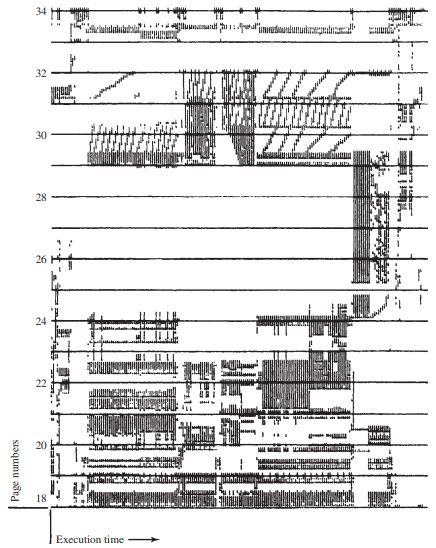
\includegraphics[width=0.5\textwidth]{images/esempio-localita.JPG}
        \label{fig:esempio-localita}
        \captionof{figure}{Esempio di località delle pagine}
    \end{minipage}
\end{Example}

\subsection*{Paginazione con memoria virtuale}

\begin{wrapfigure}{r}{0.3\linewidth}
    \vspace{-10pt}
    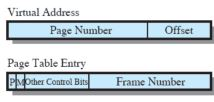
\includegraphics[width=1\linewidth]{images/page-table-entry.JPG}
    \label{fig:page-table-entry}
    \vspace{-20pt}
\end{wrapfigure}
Abbiamo visto come ogni processo ha una sua tabella delle pagine e il control block di un processo punta a tale tabella. Ogni entry della tabella contene delle informazioni aggiuntive: un bit di presenza (\verb|P|) indica se la pagina è in RAM o se bisogna prelevarla dal disco; un bit di modifica (\verb|M|) indica se la pagina è stata modificata in seguito all'ultima volta che è stata caricata in memoria principale; altri bit di controllo (\verb|Other Control Bits|); il numero di frame (\verb|Frame Number|).

In maniera più approfondita, la traduzione degli indirizzi è fatta dall'hardware, partendo da un indirizzo virtuale da cui si ottiene il numero di pagina e l'offset. Il numero di pagina va sommato con il \verb|Page Tabele Ptr|, che indica il punto di partenza della page table, e moltiplicato per il numero di bytes di ogni singola entry della tabella delle pagine. In questo modo si ottiene il numero di frame che sostituisce il numero di pagina per ottenere l'indirizzo fisico in RAM (vedi Figura \ref{fig:traduzione-indirizzi-virtuali}).\\\\
Un problema che potrebbe generarsi è che le tabelle delle pagine potrebbero contenere molti elementi, ad esempio con RAM di 1 GB, bastano 20 processi per occupare più di metà RAM con sole strutture di overhead. L'idea è di utilizzare delle tabelle delle pagine a due livelli, dove una tabella delle pagine di livello superiore punta alle tabelle delle pagine del processo. In questo sistema la traduzione degli indirizzi si complica leggermente perché l'indirizzo virtuale si spacchetta in tre parti e l'hardware deve consultare due tabelle delle pagine. La prima è indicizzata dalla prima parte dell'indirizzo e, il valore che si ottiene, va sommato con la seconda parte dell'indirizzo, che viene usato per accedere alla seconda tabella delle pagine (vedi Figura \ref{fig:traduzione-indirizzi-virtuali}).

\begin{figure}[h]
    \centering
    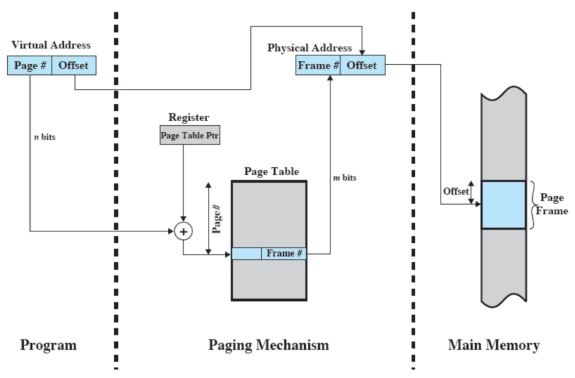
\includegraphics[width=0.49\linewidth]{images/traduzione-indirizzi-virtuali.JPG}
    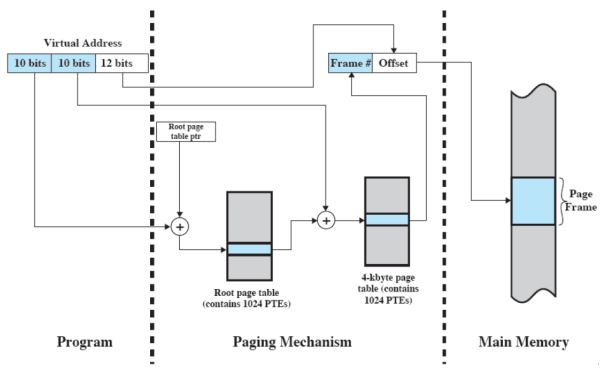
\includegraphics[width=0.5\linewidth]{images/traduzione-indirizzi-2tdp.JPG}
    \caption{Traduzione di indirizzi con una e due tabelle delle pagine}
    \label{fig:traduzione-indirizzi-virtuali}
\end{figure}

Spesso, con la memoria virtuale, viene utilizzata una memoria cache chiamata \textit{Translation Lookaside Buffer} (TLB) che contiene gli elementi delle tabelle delle pagine che sono stati usati più di recente. Questa necessità nasce dal fatto che ogni riferimento alla memoria virtuale può generare due accessi alla memoria: uno per la tabella delle pagine e uno per prendere il dato. Quindi dato un  indirizzo virtuale, il processore esamina dapprima il TLB, se la pagina è presente (\textit{TLB HIT}), si prende il frame number e
si ricava l'indirizzo reale. Altrimenti (\textit{TLB MISS}), si prende la tabella delle pagine del processo se è presente in memoria, altrimenti si gestisce il page fault come già visto. Dopodiché, il TLB viene aggiornato includendo la pagina appena acceduta usando un qualche algoritmo di rimpiazzamento se il TLB è già pieno: solitamente LRU\footnote{Least Recently Used, usato meno di recente.}.

\begin{figure}[h]
    \centering
    
\includegraphics[width=0.7\linewidth]{images/tlb.JPG}
    \caption{Funzionamento del TLB}
    \label{fig:tlb}
\end{figure}

Il TLB contiene solo alcuni elementi tratti dalle tabelle delle pagine, per questo, per trovare una specifica pagina, il sistema operativo può interrogare più elementi del TLB contemporaneamente per capire se è presente il numero di pagina desiderato. Per fare ciò c'è bisogno che il TLB contenga solo pagine in RAM.\\\\
Per quanto riguarda la dimensione delle pagine possiamo dire che più piccola è una pagina, minore è la frammentazione all'interno delle pagine ma è anche maggiore il numero di pagine per processo, il che significa che è più grande la tabella delle pagine per ogni processo. Però, allo stesso tempo, più piccola è una pagina, maggiore è il numero di pagine che si trovano in memoria principale e lo stesso processo può riuscire ad avere un resident set più grande in modo da diminuire i page fault. D'altro canto la memoria secondaria è ottimizzata per trasferire grossi blocchi di dati, e quindi per avere pagine ragionevolmente grandi. Data questa forte dualità sono stati fatti degli esperimenti per cercare il migliore valore di dimensione delle pagine e si è notato che la migliore scelta è utilizzare dimensioni delle pagine piccole.

\begin{Osservation}{Dimensione delle pagine}{}

    \begin{minipage}{\textwidth}
        \centering
        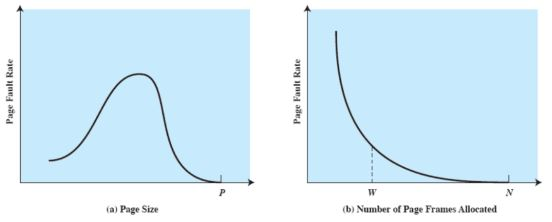
\includegraphics[width=0.7\linewidth]{images/dimensione-pagine.JPG}
        \captionof{figure}{Esperimenti sulle dimensioni delle pagine}
        \label{fig:dimensione-pagine}
    \end{minipage}
    
    Il grafico di sinistra presenta la dimensione della pagina sulle ascisse e il tasso di page fault sulle ordinate (si punta ad avere questo valore più basso possibile). Il grafico mostra un andamento a campana dove per dimensioni di pagina piccole o molto vicine alla grandezza del processo il page fault rate tende a rimanere basso, mentre verso metà processo cresce notevolmente. In realtà con pagine grandi, si ottengono pochi fault di pagina, ma allo stesso tempo si ha poca multiprogrammazione. Per questo motivo si è preferito adottare dimensioni delle pagine piccole.

    Il grafico di destra presenta il numero di page frame necessari per il processo sulle ascisse e il tasso di page fault sulle ordinate. Ovviamente, se si mettono in RAM tutte le pagine del processo (\verb|N|) non vengono generati page fault, ma allo stesso tempo non si ha lo spazio per tutti gli altri processi. Un ottimo compromesso si ottiene per \verb|W|.
\end{Osservation}


\subsection*{Segmentazione con memoria virtuale}
Abbiamo visto come la segmentazione permette al programmatore di vedere la memoria come un insieme di spazi di indirizzi, di dimensione variabile o dinamica, per semplificare la gestione delle strutture dati, per permettere di modificare e ricompilare i programmi in modo
indipendente o per condividere e proteggere i dati.

\begin{wrapfigure}{r}{0.4\linewidth}
    \vspace{-10pt}
    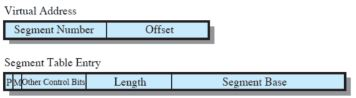
\includegraphics[width=1\linewidth]{images/segment-table-entry.JPG}
    \label{fig:segment-table-entry}
    \vspace{-20pt}
\end{wrapfigure}

Ogni processo ha una sua tabella dei segmenti e il control block di un processo punta a tale tabella. Ogni entry di questa tabella contiene: un bit (\verb|P|) per indicare se il segmento è in memoria principale; un bit (\verb|M|) per indicare se il segmento è stato modificato in seguito all'ultima volta che è stato caricato in memoria principale; la lunghezza (\verb|Lenght|) del segmento; l'indirizzo di partenza (\verb|Segment Base|) in memoria principale del segmento.

Per la traduzione degli indirizzi, il numero di segmento va sommato con il \verb|Seg Tabele Ptr|, che indica il punto di partenza della segment table, e moltiplicato per il valore di lenght della entry. In questo modo si ottiene l'indirizzo di partenza, in memoria principale, del segmento che sommato con l'offset ci dà l'indirizzo fisico (vedi Figura \ref{fig:segment-traduzione-indirizzi}).

\begin{figure}[h]
    \centering
    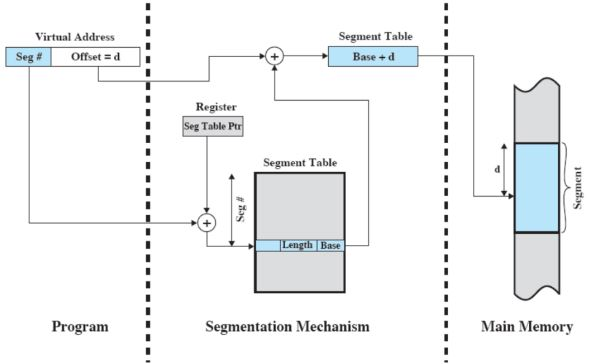
\includegraphics[width=0.7\linewidth]{images/segment-traduzione-indirizzi.JPG}
    \caption{Traduzione di indirizzi con la segmentazione}
    \label{fig:segment-traduzione-indirizzi}
\end{figure}

La paginazione è trasparente al programmatore nel senso che il programmatore non ne è (o non ne deve essere) a conoscenza. La segmentazione, invece, è visibile al programmatore, se programma in assembler, altrimenti ci pensa il compilatore ad usare i segmenti.
Tipicamente paginazione e segmentazione sono combinate, nel senso che ogni segmento viene diviso in più pagine. In questo modo si accede, con una parte di indirizzo, alla segment table, e il segmento trovato è paginato da una tabella delle pagine da cui è possibile ottenere il frame in RAM (vedi Figura \ref{fig:paginazione-segmentazione-indirizzi}).

\begin{figure}[h]
    \centering
    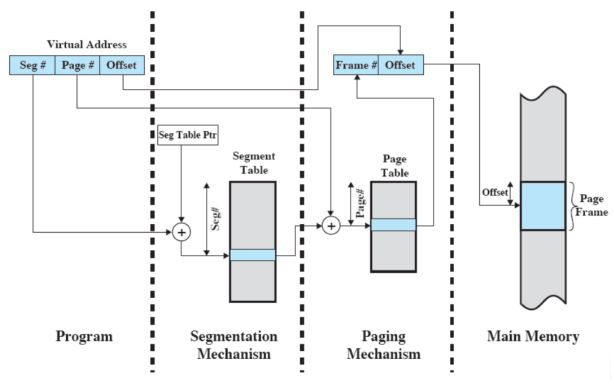
\includegraphics[width=0.7\linewidth]{images/paginazione-segmentazione-indirizzi2.JPG}
    \caption{Traduzione di indirizzi con paginazione e segmentazione}
    \label{fig:paginazione-segmentazione-indirizzi}
\end{figure}

Con la segmentazione, implementare la protezione viene naturale, dato che ogni segmento ha una base ed una lunghezza,
è facile controllare che i riferimenti siano contenuti nel giusto intervallo. Per la condivisione, basta definire un segmento che serve più processi, o al contrario che non ne serve nessuno.

\begin{Example}{Protezione e condivisione}{}

    \vspace{5pt}
    \begin{minipage}{0.4\textwidth}
        \vspace{0pt}
      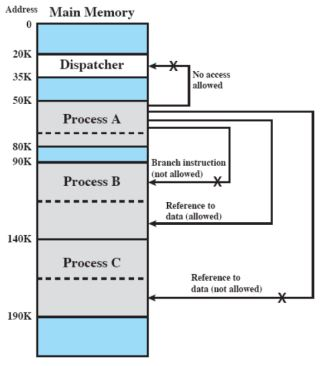
\includegraphics[width=\textwidth]{images/esempio-protezione-condivisione.JPG}
    \end{minipage}
    \hspace{10pt}
    \begin{minipage}{0.55\textwidth}
        Tre processi A, B, C sono divisi in una parte privata (quella più in altro) e in una pubblica (quella più in basso). Ad esempio la parte privata di A non può eseguire un branch nella parte privata di un altro processo, ma può far riferimento ai dati pubblici del processo B.

        Sta al programmatore la scelta di quali parti dei processi A, B e C siano condivise e quali no.
    \end{minipage}
\end{Example}

\section{Memoria virtuale e sistema operativo}
Quando il sistema operativo deve decidere se utilizzare la paginazione e/o la segmentazione deve definire: una politica di prelievo (\textit{fetch policy}); una politica di posizionamento (\textit{placement policy}); una politica di sostituzione (\textit{replacement policy}); altro (gestione del resident set, politica di pulitura, controllo del carico). Per ogniuna di queste politiche ci sono degli algoritmi che cercano di minimizzare i page fault.

\subsection*{Fetch policy}
La politica di prelievo decide quando una pagina debba essere portata in memoria principale. Si usano principalmente due politiche:
\begin{itemize}
    \item con la paginazione su richiesta (\textit{demand paging}) una pagina viene portata in memoria principale nel momento in cui un qualche processo la richiede, generando molti page fault nei primi momenti di vita del processo;
    \item la prepaginazione (\textit{prepaging}) cerca di anticipare le richieste del processo portando in memoria principale più pagine di quelle richieste sfruttando il principio di località.
\end{itemize}

\subsection*{Placement policy}
La politica di posizionamento decide dove mettere una pagina in memoria principale quando c'è almeno un frame libero. Tipicamente, si sceglie il primo frame libero ma, in realtà, può essere messa in qualunque spazio libero grazie alla presenza dell'hardware per la traduzione degli indirizzi.

\subsection*{Replacement policy}
La politica di sostituzione decide quale pagina sostituire nel caso in cui tutti i frame della RAM sono occupati. Il tutto va fatto in modo da minimizzare la probabilità che la pagina appena sostituita venga subito richiesta di nuovo.
Bisogna tener presente che se un frame è bloccato (\textit{Frame Locking}), non si può sostituire, ad esempio i frame a livello di kernel del sistema operativo.

Gli algoritmi di sostituzione che si possono utilizzare sono: sostituzione della pagina usata meno di recente (LRU), sostituzione a coda (FIFO), sostituzione ad orologio (clock).

\begin{Example}{Algoritmi di sostituzione}{}
    \textit{Supponiamo di avere 3 frame in memoria principale e la seguente sequenza di richieste delle pagine:}
    \begin{equation*}
        2,\mbox{ }3,\mbox{ }2,\mbox{ }1,\mbox{ }5,\mbox{ }2,\mbox{ }4,\mbox{ }5,\mbox{ }3,\mbox{ }2,\mbox{ }5,\mbox{ }2
    \end{equation*}
    Analizziamo il comportamento degli algoritmi di sostituzione delle pagine, sulla base della sostituzione ottima che rappresenta la soluzione migliore da utilizzare quando si conosce l'esito di un esperimento:
    \begin{itemize}
        \item La \textit{soluzione ottimale} è quella che sostituisce la pagina che verrà richiesta più in là nel futuro. Ovviamente, non è implementabile ma è definita per fare i successivi confronti sperimentali che dovranno avvicinarsi il più possibile ai 3 page fault generati da questo algoritmo;
        
        \begin{minipage}{\textwidth}
            \centering
            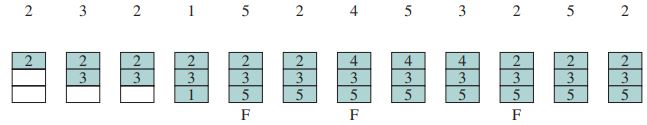
\includegraphics[width=0.7\linewidth]{images/esempio-sostituzione-ottimale.JPG}
            \label{fig:esempio-sostituzione-ottimale}
        \end{minipage}
        
        \item La \textit{sostituzione LRU} sostituisce la pagina in cui non sia stato fatto riferimento per il tempo più lungo, basandosi sul principio di località, dovrebbe essere la pagina che ha meno probabilità di essere usata nel prossimo futuro. Il problema di questa soluzione è che la sua implementazione è problematica perché occorre etichettare ogni frame con il tempo dell'ultimo accesso;

        \begin{minipage}{\textwidth}
            \centering
            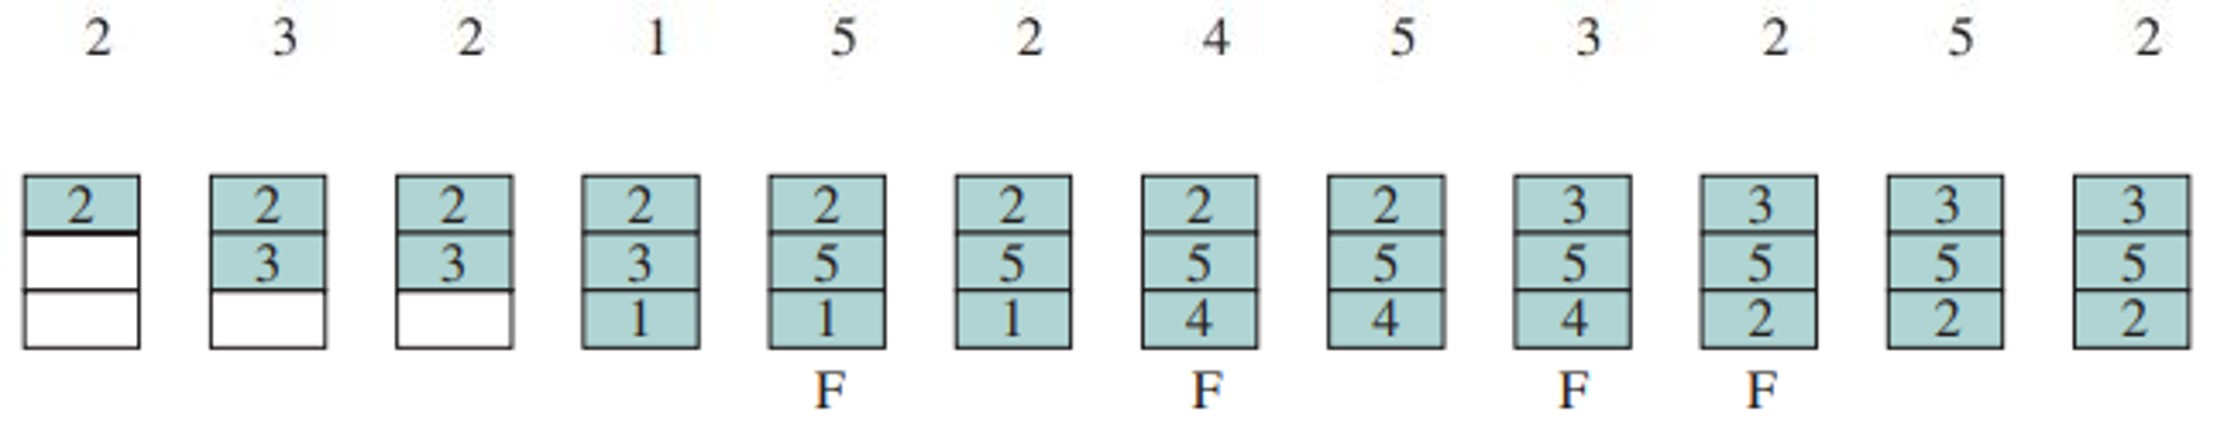
\includegraphics[width=0.7\linewidth]{images/esempio-sostituzione-lru.JPG}
            \label{fig:esempio-sostituzione-lru}
        \end{minipage}

        \item Nella \textit{sostituzione FIFO} i frame allocati ad un processo sono trattati come una coda circolare, da cui le pagine vengono rimosse a turno (round robin). In questo modo si rimpiazzano le pagine che sono state in memoria per più tempo anche se potrebbero servire nel breve termine;

        \begin{minipage}{\textwidth}
            \centering
            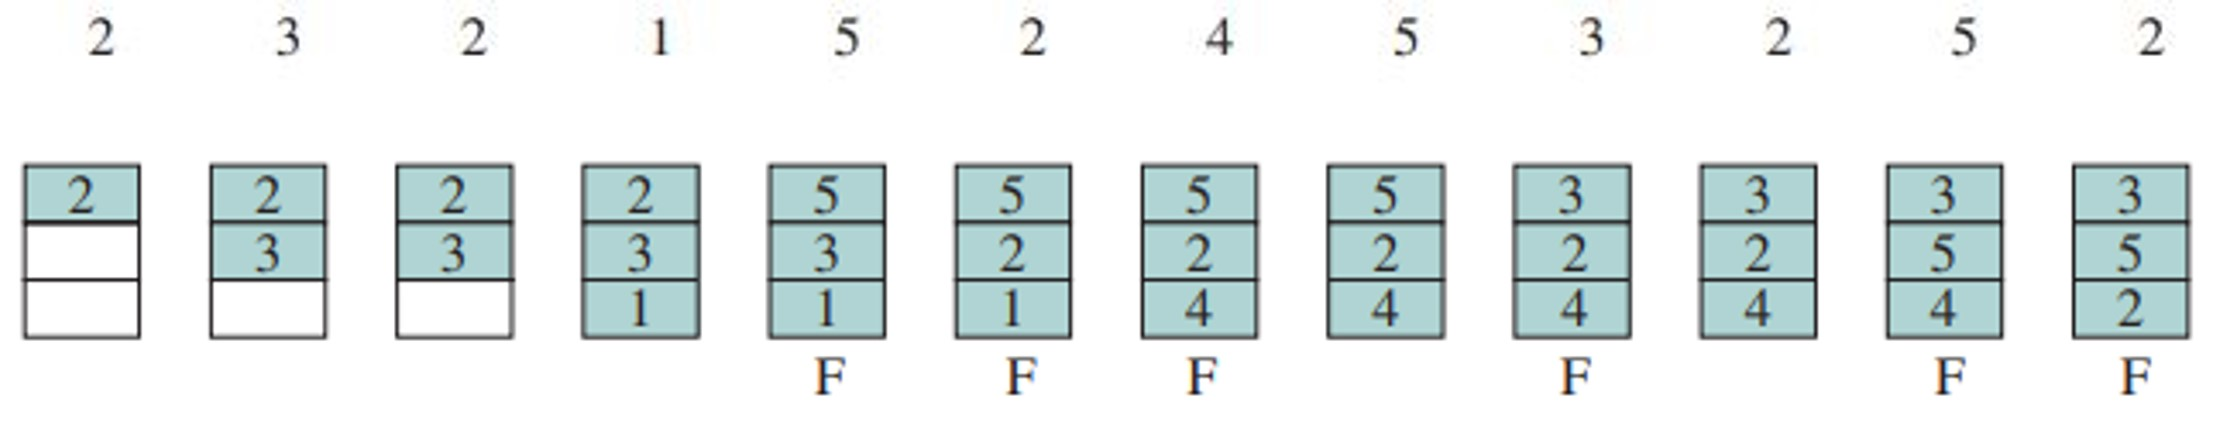
\includegraphics[width=0.7\linewidth]{images/esempio-sostituzione-fifo.JPG}
            \label{fig:esempio-sostituzione-fifo}
        \end{minipage}

        \item La \textit{sostituzione a clock} è un compromesso tra LRU e FIFO, ovvero c'è uno \verb|use bit| per ogni frame, che indica se la pagina è stata riferita di recente. Questo bit è settato ad 1 quando la pagina viene caricata in memoria principale, e poi rimesso ad 1 per ogni accesso al suo interno. Quando occorre sostituire una pagina, il sistema operativo cerca come nella FIFO, e seleziona il frame contenente la pagina che ha per prima lo use bit a 0, se nel frattempo incontra una pagina che lo ha a 1, lo mette a 0 e procede con la prossima.
        
        Questo algoritmo è alla base di molti algoritmi di sostituzione delle pagine attualmente utilizzati nei sistemi operativi. Con * viene indicato lo \verb|use bit| a 1, mentre senza è a 0:

        \begin{minipage}{\textwidth}
            \centering
            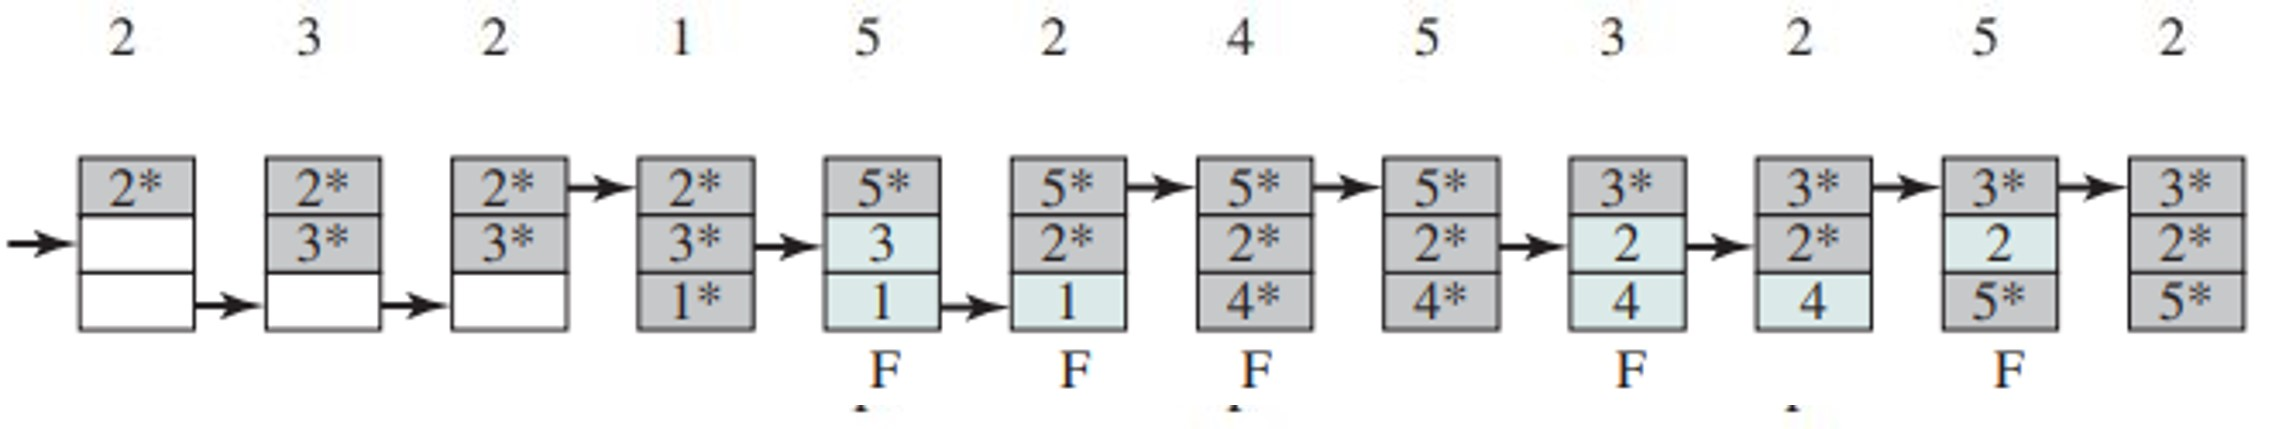
\includegraphics[width=0.7\linewidth]{images/esempio-sostituzione-clock.JPG}
            \label{fig:esempio-sostituzione-clock}
        \end{minipage}
    \end{itemize}

    Di seguito un confronto grafico sulle prestazioni degli algoritmi analizzati:
    
    \begin{minipage}{\textwidth}
            \centering
            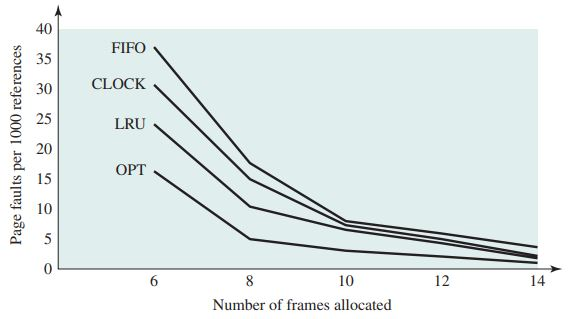
\includegraphics[width=0.7\linewidth]{images/confronto-algoritmi-sostituzione.JPG}
            \label{fig:confronto-algoritmi-sostituzione}
            \captionof{figure}{Confronto degli algoritmi di sostituzione}
        \end{minipage}
\end{Example}

Un'altra tecnica che viene spesso utilizzata è il \textit{page buffering}, dove si toglie un pò di memoria al processo per utilizzarla per salvare la pagina in una cache prima di rimpiazzarla. In questo modo se poi viene nuovamente referenziata, si può subito riportarla in memoria.

\subsection*{Gesione del resident set}
La gestione del resident set risponde a due necessità: 
\begin{itemize}
    \item per ogni processo in esecuzione, quanti frame di RAM vanno allocati (\textit{resident set management})? Si possono utilizzare due approcci: o si fa un'allocazione fissa decidendo il numero di frame necessari durante la creazione di un processo, oppure, con allocazione dinamica il numero di frame varia durante la vita del processo in base alle statistiche raccolte.
    \item quando si rimpiazza un frame, bisogna scegliere solo tra i frame che appartengono al processo corrente, oppure si può sostituire un frame qualsiasi (\textit{replacement scope})? Anche in questo caso ci sono due approcci: si utilizza una politica locale rimpiazzando un frame con uno dello stesso processo o, al contrario, con la politica globale si può scegliere un frame di qualsiasi processo.
\end{itemize}

\subsection*{Politica di pulitura}
Se un frame è stato modificato, va riportata la modifica anche sulla pagina corrispondente non appena avviene la modifica oppure non appena il frame viene sostituito. Si fa tipicamente una via di mezzo, intrecciata con il page buffering, dove si raccolgono un pò di richieste di frame da modificare e si eseguono insieme così da essere più efficienti.

\subsection*{Controllo del carico}
Il controllo del carico, con il medium-term scheduler, cerca di avere il numero più alto possibile di processi attivi, ma senza arrivare al thrashing, perché se ci sono troppi processi i resident set diventano troppo piccoli e si generano troppi page fault. Si aumentano e diminuiscono i processi attivi gestendo opportunamente gli stati Suspend e Non-Suspend attraverso delle politiche di monitoraggio.

\section{Gestione della memoria in Linux}
In Linux si ha una distinzione netta tra richieste di memoria da parte del kernel e quelle dei processi utente, questo perché Linux si fida del kernel e fa pochi controlli, se non nessuno, per questo tipo di richieste. Per i processi utente, invece, sono necessari dei controlli di protezione e di rispetto dei limiti assegnati. Il kernel può usare sia la memoria a lui riservata che quella normalmente usata dai processi utente e le richieste di memoria del kernel sono ottimizzate sia per le richieste piccole che per le grandi: se la richiesta è piccola (pochi bytes), fa in modo di avere alcune pagine già pronte da cui può prendere i pochi bytes richiesti (slab allocator); se la richiesta è grande (fino a 4MB), fa in modo di allocare più pagine contigue in frame contigui utilizzando il buddy system.

In Linux vengono utilizzate la fetch policy di paging on demand, il placement policy con il primo frame libero e il replacement policy con l'algoritmo dell'orologio, anche se il kernel più recente usa un LRU “corretto”. Per l'algoritmo di clock si usano due flag in ogni entry delle page table: \verb|PG_referenced| (pagine referenziate) e \verb|PG_active| (pagine attive). Sulla base di \verb|PG_active|, il kernel mantiene due liste di pagine: attive ed inattive. Il \verb|kswapd| è un kernel thread in esecuzione periodica, che scorre solo le pagine inattive. Il \verb|PG_referenced| è settato quando la pagina viene richiesta, dopodiché o arriva prima \verb|kswapd| o un altro riferimento. Nel primo caso viene settata la pagina attiva, nel secondo il \verb|PG_referenced| di nuovo a zero. In questo sistema solo le pagine inattive possono essere rimpiazzate.

La gestione del resident set avviene con una politica dinamica con replacement scope globale, anche qui, c'è un buddy system per richieste grandi. La politica di pulitura è ritardata il più possibile e le scritture vengono effettuate o quando la page cache è troppo piena con molte richieste pending, o si hanno troppe pagine sporche da troppo tempo, oppure si ha una richiesta esplicita di un processo (\verb|flush|, \verb|sync| o simili). Infine il controllo del carico è totalmente assente.
